\documentclass[a4paper]{article}
\usepackage[english]{babel}
\usepackage[utf8]{inputenc}
\usepackage{amsmath}
\usepackage{graphicx}
\usepackage[colorinlistoftodos]{todonotes}
\usepackage{xeCJK}
\usepackage{abstract}
\usepackage[CJKbookmarks=true]{hyperref}
\usepackage{setspace}
\renewcommand{\baselinestretch}{1.3}
\usepackage{subfigure}
\usepackage{minted}


\title{模式识别\\基于深度学习的海狮种群数量识别}
\author{第八组\\16121536 陈悦\\16121674 苗伟华} % 大家自己写下学号姓名 
\date{}
\begin{document}
\maketitle

\tableofcontents
\thispagestyle{empty}
\newpage

\renewcommand{\abstractname}{摘要}
\thispagestyle{empty}
\begin{onecolabstract}
Enter a short summary here. What topic did you want to investigate and why? What experiment did you perform? What were your main results and conclusion?
\end{onecolabstract}
\newpage
\setcounter{page}{1}
\section{题目描述}
\label{sec:introduction}

Write a short introduction about what you did in the lab.

Briefly explain what methods you will use in the experiment, and what values you will extract from the data.

If you want to cite something you can do it like this\cite{nano3}, this will refer to the medium defined in the end that has the tag nano3.

\section{背景}
\label{sec:theory}

\subsection{this is how you make a subsection}
No theory really needed for this experiment.

\section{解决思路}

\subsection{数据预处理}

\begin{figure}[htbp]
\centering
\begin{minipage}[t]{0.48\textwidth}
\centering
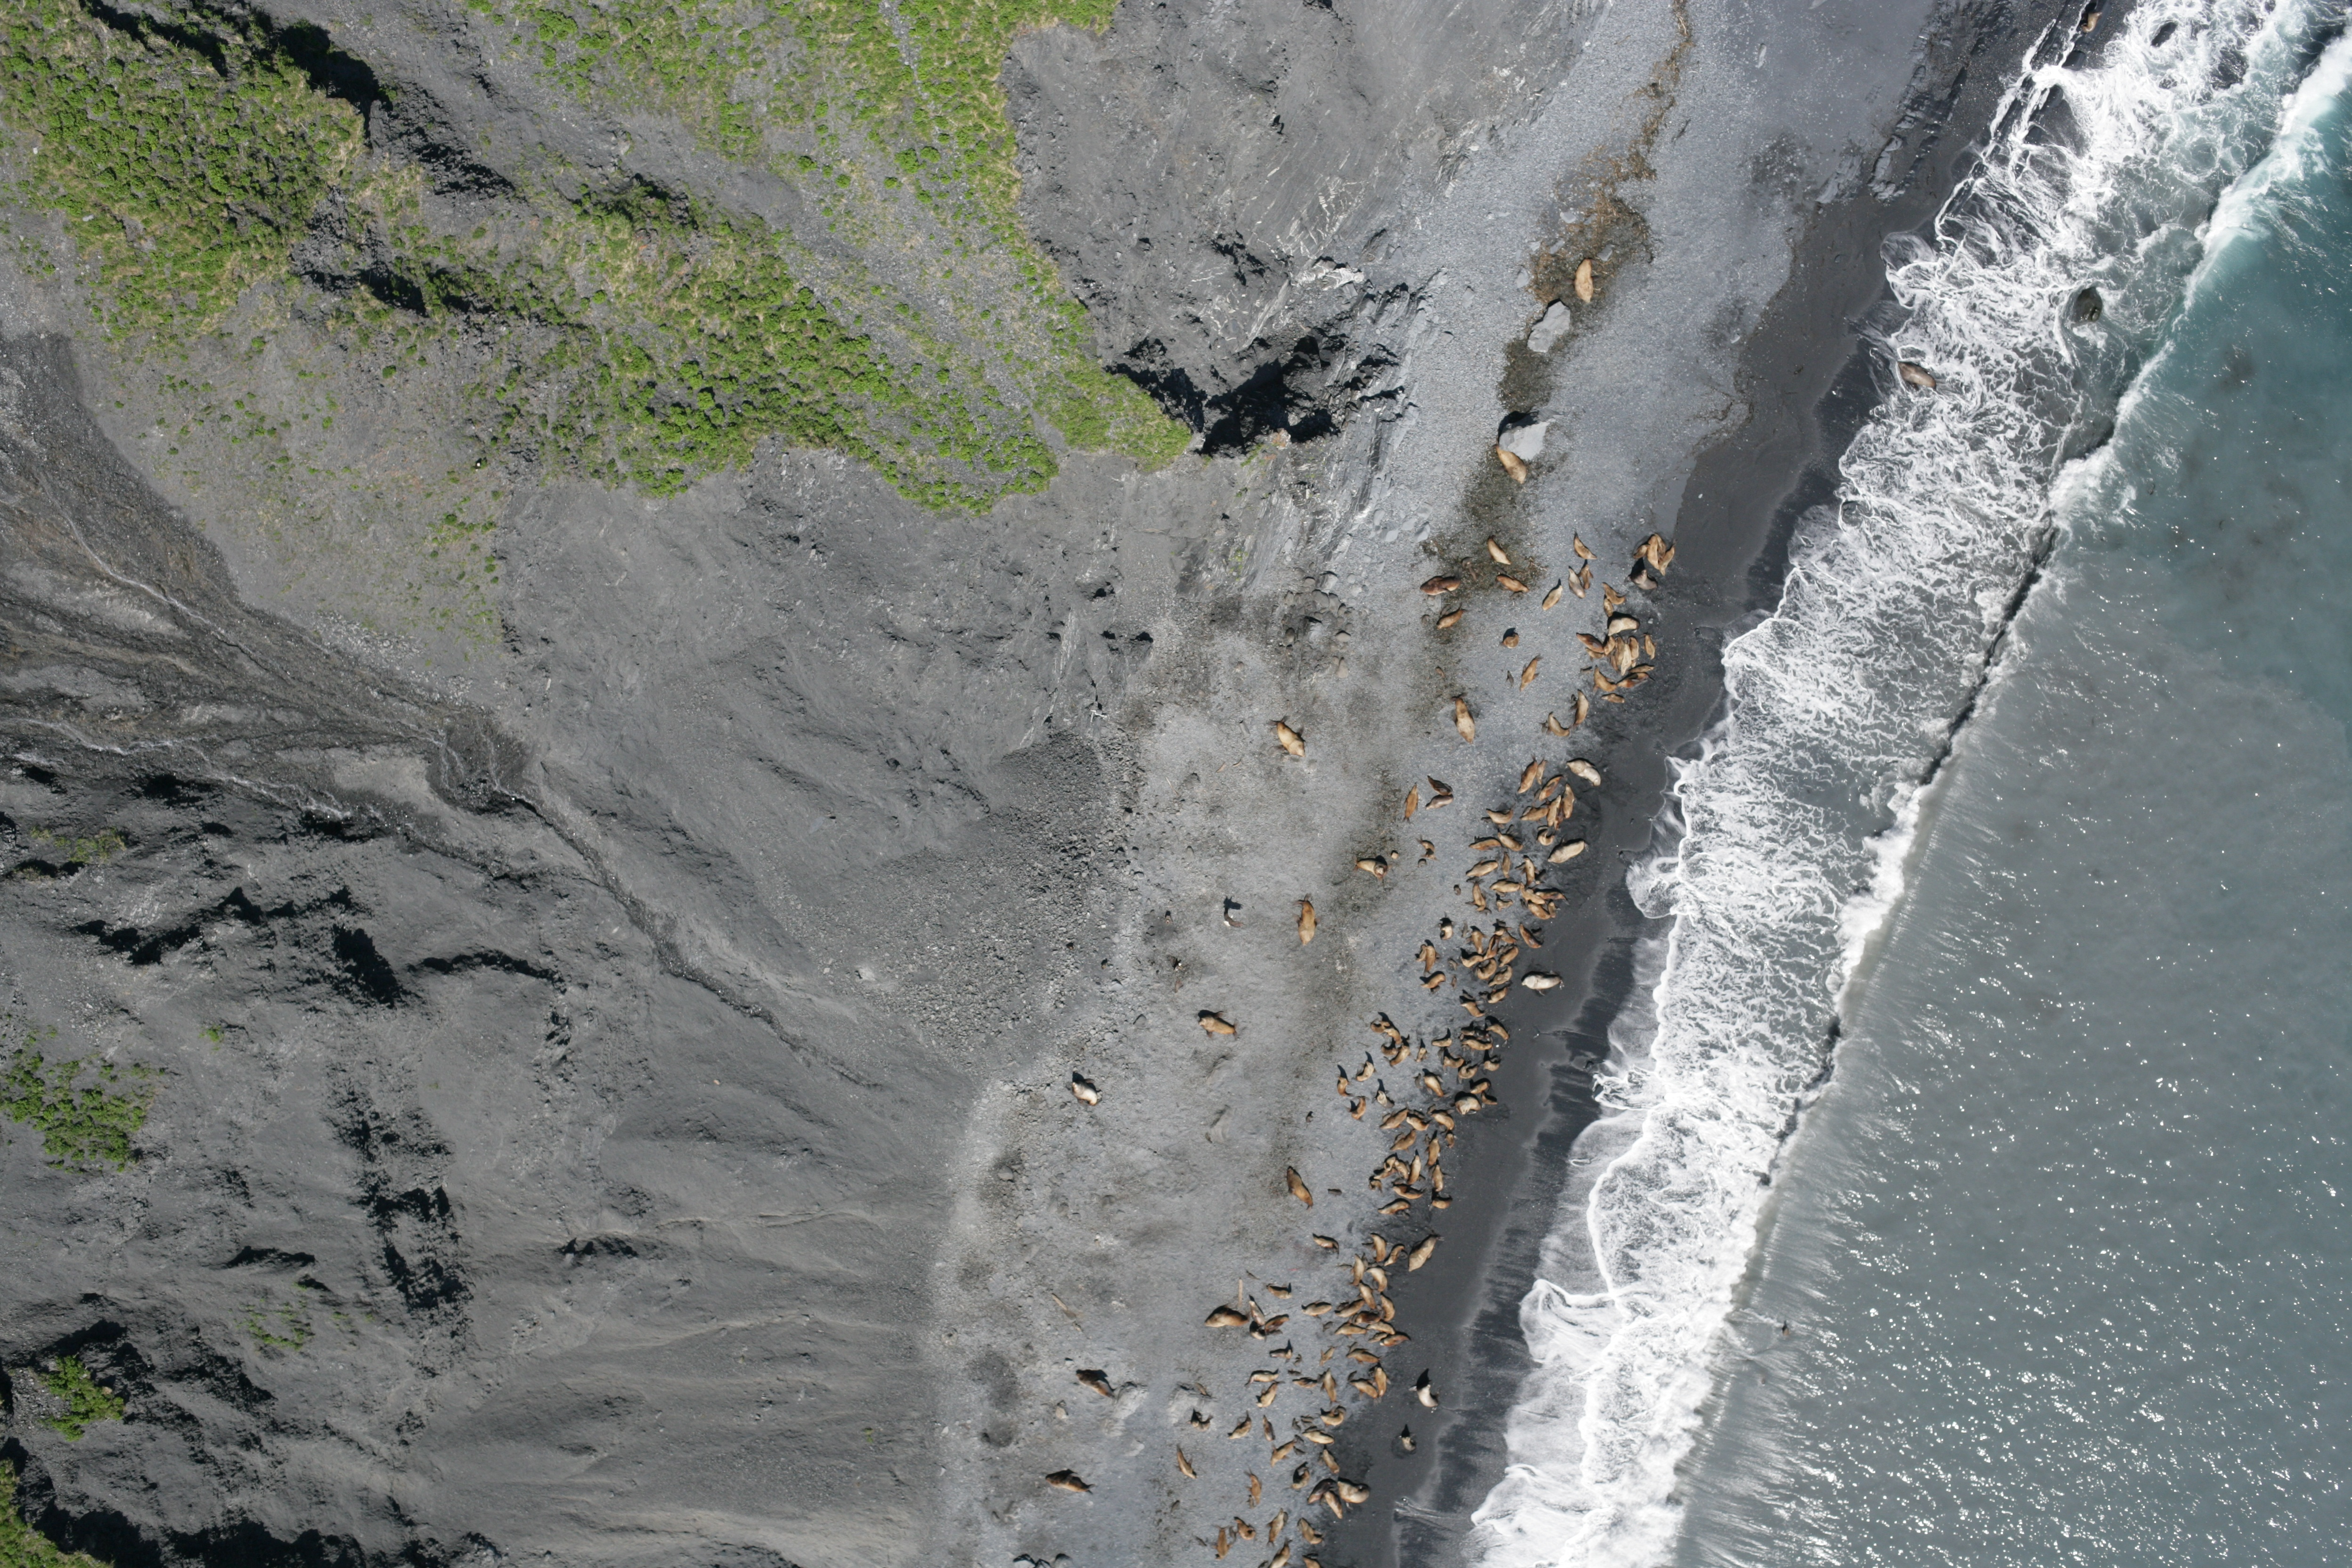
\includegraphics[scale=0.03]{41.jpg}
\caption{原始图像}
\end{minipage}
\begin{minipage}[t]{0.48\textwidth}
\centering
\includegraphics[scale=0.03]{41dotted.jpg}
\caption{标记后的图像}
\end{minipage}
\end{figure}


因为每张照片的分辨率达到$5k$,直接训练效果会很差,因此我们将一张照片分割成若干张$300 \times 300$分辨率的图片。这样原本一张照片经过分割之后可以变成二十到三十张图片,大大增加了数据量,同时使得训练效果增强。(见 Figure \ref{f1})

\begin{minted}{python}
def cutFigure(image, res, h, w):
    # 将图片重置大小,保证平均分割
    img = cv2.resize(image, (int(w*r), int(h*r)))
    h1, w1, d = img.shape
    trainX = []
    trainY = []
    for i in range(int(w1//width)):
        for j in range(int(h1//width)):
            # 分割好的图片放入trainX中
            trainX.append(img[j*width:j*width+width, i*width:i*width+width, :])
            # 分割好的图片中,各种标记点的数量放到trainY中
            trainY.append(res[i, j, :])
    return np.array(trainX), np.array(trainY)
\end{minted}

\begin{figure}[htbp]
\centering
\begin{minipage}[t]{0.48\textwidth}
\centering
\includegraphics[scale=0.5]{sample1.png}
\end{minipage}
\begin{minipage}[t]{0.48\textwidth}
\centering
\includegraphics[scale=0.5]{sample2.png}
\end{minipage}
\caption{分割后的图像}
\label{f1}
\end{figure}

人工标记会在不同海狮身上标注不同的颜色点,因此我们的第一步是要提取每个小图片中各个颜色的数量。
将背景变成黑色,只留下标记的颜色点。(见 Figure \ref{f2})

\begin{minted}{python}
origin = cv2.imread(path1) # 原始图像
originDotted = cv2.imread(path2) # 标记后的图像
img1 = cv2.GaussianBlur(origin, (5, 5), 0)  # 高斯滤波,用于去除高斯噪声

# 取原始图像和标记后图像之差的绝对值
absdiff = cv2.absdiff(origin, originDotted)
# 将背景置为黑色,只保留标记点
mask_1 = cv2.cvtColor(origin, cv2.COLOR_BGR2GRAY)
mask_1[mask_1 < 50] = 0
mask_1[mask_1 > 0] = 255
dotImg = cv2.bitwise_or(absdiff, absdiff, mask=mask_1)
\end{minted}

然后将图片转化成灰度图,并用斑点检测技术(能够在较暗/亮背景下检测出亮/暗区域)得到每个标记点的颜色,最后统计出每种颜色的数量。

\begin{minted}{python}
# 转换成灰度图,进行斑点检测
grayImg = np.max(dotImg, axis=2)
blobs = skimage.feature.blob_log(
    grayImg, min_sigma=3, max_sigma=7, num_sigma=1, threshold=0.05)
# blob 或者叫斑点,就是在一幅图像上,暗背景上的亮区域。或者亮背景上的暗区域,都能够称为blob
h, w, d = originDotted.shape
res = np.zeros(
    (int((w*r)//width)+1, int((h*r)//width)+1, 5), dtype='int16')

for blob in blobs:
    # 斑点的坐标
    y, x, s = blob
    # 得到斑点中心的rgb的值(颜色)
    b, g, R = img1[int(y)][int(x)][:]
    x1 = int((x*r)//width)
    y1 = int((y*r)//width)
    # 根据rgb值判断颜色
    if R > 225 and b < 25 and g < 25:  # RED
        res[x1, y1, 0] += 1
    elif R > 225 and b > 225 and g < 25:  # MAGENTA
        res[x1, y1, 1] += 1
    elif R < 75 and b < 50 and 150 < g < 200:  # GREEN
        res[x1, y1, 4] += 1
    elif R < 75 and 150 < b < 200 and g < 75:  # BLUE
        res[x1, y1, 3] += 1
    elif 60 < R < 120 and b < 50 and g < 75:  # BROWN
        res[x1, y1, 2] += 1
\end{minted}

\begin{figure}[htbp]
\centering
\begin{minipage}[t]{0.48\textwidth}
\centering
\includegraphics[scale=0.5]{sampe1Dotted.png}
\end{minipage}
\begin{minipage}[t]{0.48\textwidth}
\centering
\includegraphics[scale=0.5]{sample2Dotted.png}
\end{minipage}
\caption{提取标记点后的图像}
\label{f2}
\end{figure}

按照上述方法处理完所有照片后,我们可以将得到样本分为训练集与测试集,方便接下来调参的进行。




\section{结果}

\subsection{Resistor}


Show the 2 graphs for transistor behavior as asked for in the manual.

\begin{figure}
\centering
\includegraphics[width=1\textwidth]{elephant.png}
\caption{\label{fig:data1}Replace this figure \cite{elephant} with the one you've made and add an appropriate caption. }
\end{figure}

\subsection{Transistor}
Include the two 2D plots you made about the behavior of the resistor. Most of the time \LaTeX doesn't put the figures where you would expect them but where they are ideally place from a layout prospective, you can always just refer to the number of the picture with the label command for example Figure \ref{fig:data}.

\begin{figure}
\centering
\includegraphics[width=0.5\textwidth]{circuit_diagram.png}
\caption{\label{fig:data}Replace this figure  \cite{xkcd} with the one you've made and add an appropriate caption. By the way you should always cite when you put any stuff in your reports you didn't make yourself.}
\end{figure}



\newpage
\section{Some LaTeX tips}
\label{sec:latex}
\subsection{How to Include Figures}

First you have to upload the image file (JPEG, PNG or PDF) from your computer to writeLaTeX using the upload link the project menu. Then use the includegraphics command to include it in your document. Use the figure environment and the caption command to add a number and a caption to your figure. See the code for Figure \ref{fig:frog} in this section for an example.

\begin{figure}
\centering
\includegraphics[width=0.3\textwidth]{frog.jpg}
\caption{\label{fig:frog}This frog was uploaded to writeLaTeX via the project menu.}
\end{figure}

\subsection{How to Make Tables}

Use the table and tabular commands for basic tables --- see Table~\ref{tab:widgets}, for example.

\begin{table}
\centering
\begin{tabular}{l|r}
Item & Quantity \\\hline
Widgets & 42 \\
Gadgets & 13
\end{tabular}
\caption{\label{tab:widgets}An example table.}
\end{table}

\subsection{How to Write Mathematics}

\LaTeX{} is great at typesetting mathematics. Let $X_1, X_2, \ldots, X_n$ be a sequence of independent and identically distributed random variables with $\text{E}[X_i] = \mu$ and $\text{Var}[X_i] = \sigma^2 < \infty$, and let

\begin{equation}
S_n = \frac{X_1 + X_2 + \cdots + X_n}{n}
      = \frac{1}{n}\sum_{i}^{n} X_i
\label{eq:sn}
\end{equation}

denote their mean. Then as $n$ approaches infinity, the random variables $\sqrt{n}(S_n - \mu)$ converge in distribution to a normal $\mathcal{N}(0, \sigma^2)$.

The equation \ref{eq:sn} is very nice.

\subsection{How to Make Sections and Subsections}

Use section and subsection commands to organize your document. \LaTeX{} handles all the formatting and numbering automatically. Use ref and label commands for cross-references.

\subsection{How to Make Lists}

You can make lists with automatic numbering \dots

\begin{enumerate}
\item Like this,
\item and like this.
\end{enumerate}
\dots or bullet points \dots
\begin{itemize}
\item Like this,
\item and like this.
\end{itemize}
\dots or with words and descriptions \dots
\begin{description}
\item[Word] Definition
\item[Concept] Explanation
\item[Idea] Text
\end{description}

We hope you find write\LaTeX\ useful, and please let us know if you have any feedback using the help menu above.

\begin{thebibliography}{9}
\bibitem{nano3}
  K. Grove-Rasmussen og Jesper Nygård,
  \emph{Kvantefænomener i Nanosystemer.
  Niels Bohr Institute \& Nano-Science Center, Københavns Universitet}

\bibitem{elephant}
  How to fit an elephant,
  \emph{https://www.johndcook.com/blog/2011/06/21/how-to-fit-an-elephant/}
  
\bibitem{xkcd}
  xkcd 730,
  \emph{https://xkcd.com/730/}

\end{thebibliography}
\end{document}